\section{Grad-CAM}
Grad-CAM is a white box method. The main parameter for this method is which layer that should be analyzed.

There are many existing implementations for this method, some of them using the PyTorch library.

TODO: how does it work?


\begin{figure}[H]
\centering
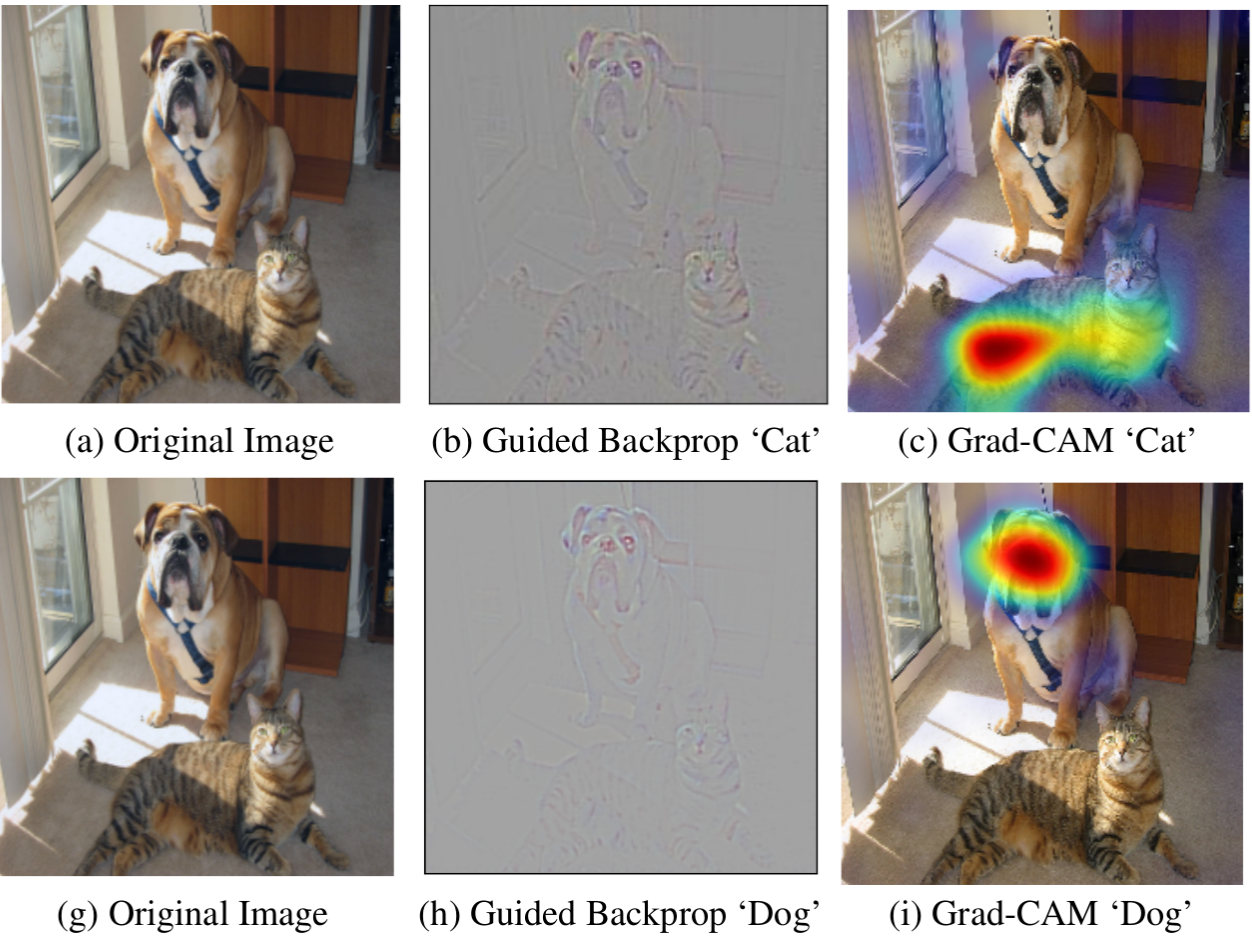
\includegraphics[width=12cm]{chapters/02_methods/images/grad-cam-example.png}
\caption{Grad-CAM explaining classes "cat" and "dog"}
\end{figure}






\begin{figure}[H]
\centering
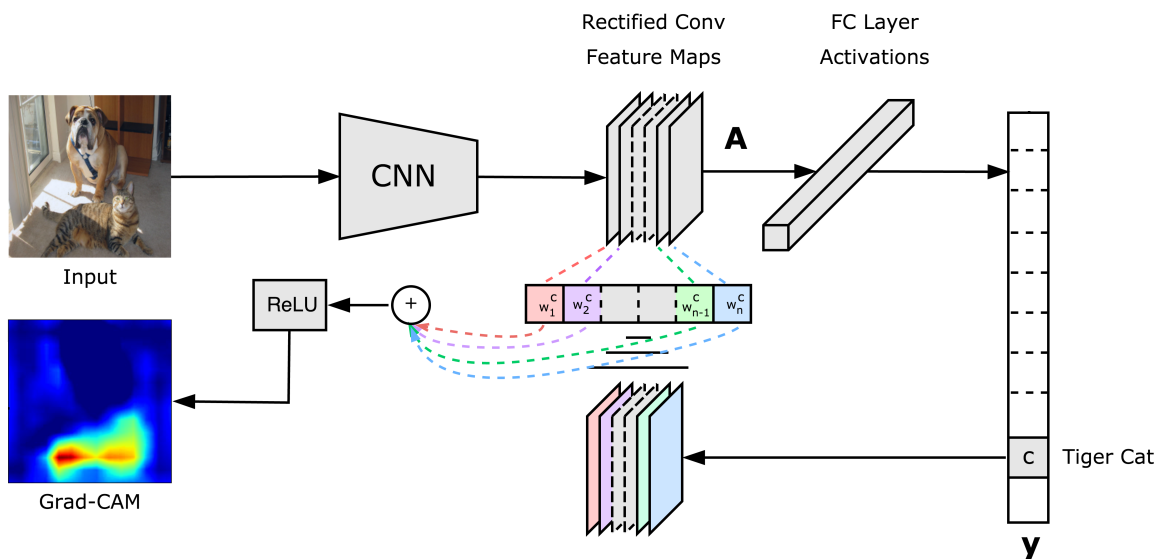
\includegraphics[width=12cm]{chapters/02_methods/images/grad-cam.png}
\caption{Grad-CAM explanation}
\end{figure}


* works on a specific layer of the neural network
* get feature map for every channel of this layer
* sum up feature map
* based on output class, so activation has to flow backwards

So, to explain in simple terms, we simply take the final convolutional feature map and then we weigh every channel in that feature with the gradient of the class with respect to the channel. It’s just nothing but how intensely the input image activates different channels by how important each channel is with regard to the class. The best part is it doesn’t require any re-training or change in the existing architecture.